\documentclass[xcolor=x11names,table]{beamer}

\usepackage{myDefaultPackageSetup/Beamer/myDefaultsBeamer}
\ProvidesPackage{myTheme1}

\usetheme{Madrid}
\setbeamercolor{title}{fg=white}
\setbeamercolor*{subtitle}{fg=white}

\setbeamercolor{section title}{fg=white,bg=blue!30}
\setbeamercolor{subsection title}{fg=white,bg=blue!30}
\setbeamercolor{subsubsection title}{fg=white,bg=blue!30}

\beamertemplatenavigationsymbolsempty
\setbeamertemplate{frame numbering}[fraction]
\AtBeginSection[]{
  \begin{frame}
  \vfill
  \centering
  \begin{beamercolorbox}[sep=8pt,center,shadow=true,rounded=true]{section title}
    \usebeamerfont{section title}\insertsectionhead\par%
  \end{beamercolorbox}
  \vfill
  \end{frame}
}
\AtBeginSubsection{
    \begin{frame}
    \centering
    {\usebeamerfont{subsection name}\usebeamercolor[fg]{subsection %
    name}\subsectionname~\insertsubsectionnumber}%
    \vskip1em\par
    \begin{beamercolorbox}[sep=4pt,center,shadow=true,rounded=true]{subsection title}
      \usebeamerfont{subsection title}\insertsubsection\par
    \end{beamercolorbox}
    \end{frame}
}
\AtBeginSubsubsection{
    \begin{frame}
    \centering
    {\usebeamerfont{subsubsection name}\usebeamercolor[fg]{subsubsection %
    name}\subsubsectionname~\insertsubsubsectionnumber}%
    \vskip1em\par
    \begin{beamercolorbox}[sep=4pt,center,shadow=true,rounded=true]{susubsection title}
      \usebeamerfont{subsection title}\insertsubsubsection\par
    \end{beamercolorbox}
    \end{frame}
}
% Section numbering
\setbeamertemplate{section in toc}[sections numbered]
\setbeamertemplate{subsection in toc}[subsections numbered]
\makeatletter
\setbeamertemplate{section page}{
  \centering
  \begin{minipage}{22em}
    \raggedright
    \usebeamercolor[fg]{section title}
    \usebeamerfont{section title}
    \thesection. \insertsectionhead\\[-1ex]
    \usebeamertemplate*{progress bar in section page}
    \par
    \ifx\insertsubsectionhead\@empty\else%
      \usebeamercolor[fg]{subsection title}%
      \usebeamerfont{subsection title}%
      \thesection. \thesubsection.\insertsubsectionhead
    \fi
  \end{minipage}
  \par
  \vspace{\baselineskip}
}
\makeatother


%%%%%%%%%%%%%%%%%%%%%%%%%%%%%%%%%%%%%
%       Show notes on pympress      %
%%%%%%%%%%%%%%%%%%%%%%%%%%%%%%%%%%%%%
%\usepackage{pgfpages}
%\setbeamertemplate{note page}[plain]
%\setbeameroption{show notes on second screen=right}
%%\setbeameroption{show only notes}

\title[\textcolor{white}{Third Milestone}]
{Group A3 - Big Brother: Third Milestone}
\author{Group A3}
\institute[TU Berlin]{TU Berlin}
\date{\today}

\begin{document}
\begin{frame}
\titlepage
\end{frame}

\begin{frame}{Table of contents}
\tableofcontents
\end{frame}



\section{Logic}

\title[\textcolor{white}{Milosz}]{}
\subsection{Video training (eduVid)}
\begin{frame}{Motivation \& Overview}
\begin{itemize}
    \item Step 1: Summary of the issues of recorded classes in the form of
    indexes.
    \item Step 2: Informed learning.
    \item Step 3: Conveniently switch between specific topics on 
    which the student wants to focus more or repeat.
\end{itemize}
\end{frame}

\begin{frame}{Python modules}
\begin{itemize}
    \item OpenCV
    \item Tesseract
    \item The Natural Language Toolkit (NLTK)
    \item Rapid Automatic Keyword Extraction (RAKE)
    \item VLC
\end{itemize}
\end{frame}

\begin{frame}{Pipeline process}
\begin{enumerate}
    \item Script extraction
    \item Summarization
    \item Extraction of keywords
    \item Recognizing the change of presentation slides and recognizing
    the content on them using OCR
    \item If keyword from script $=$ keyword from presentation -
    index
    \item Access to relevant segments by demand
    \item Use a knowledge graph to make the program work more efficiently
    - (keywords are not always used when talking about a given topic)
\end{enumerate}
\end{frame}

\begin{frame}{Demo}
We are going to demonstrate the following functionalities:
\begin{itemize}
    \item video footage processing (from presentation till text)
    \item video player
\end{itemize}
\end{frame}

\title[\textcolor{white}{Nurali}]{}
\subsection{Face and Gesture recognition}

\section{Frontend}
\begin{frame}{Progress report}
\begin{itemize}
    \item Meet the teams: Added names of team members
    \item Login camera: 
    \begin{itemize}
        \item countdown to take picture
        \item image download
    \end{itemize}
    \item Bug fixes
    \item configure GPU server
\end{itemize}
\end{frame}

\begin{frame}{TODOs}
\begin{itemize}
    \item Getting docker container to work (already started)
    \item Face recognition \arrow compare live image with backend image
    \item Adding pictures to our team
    \item Interface for eduVid-team
\end{itemize}
\end{frame}

\title[\textcolor{white}{Mike}]{}
\section{Database \& Benchmarking}

\subsection{Database}
\begin{frame}{Progress report}
\begin{itemize}
    \item Fixed potential problems with concurrency
    \item Implement some further tests
    \item Implement user encoding functions
    \item Inserted more user data into database
\end{itemize}
\end{frame}

\begin{frame}{TODOs}
\begin{itemize}
    \item calculate encodings for user data in database
    \item implement requests regarding features of eduVid group
\end{itemize}
\end{frame}

\subsection{Benchmarking}
\begin{frame}{Progress}
\begin{itemize}
    \item Clean up
    \item Bug fixes 
    \item Change deprecated methods
\end{itemize}
\begin{center}
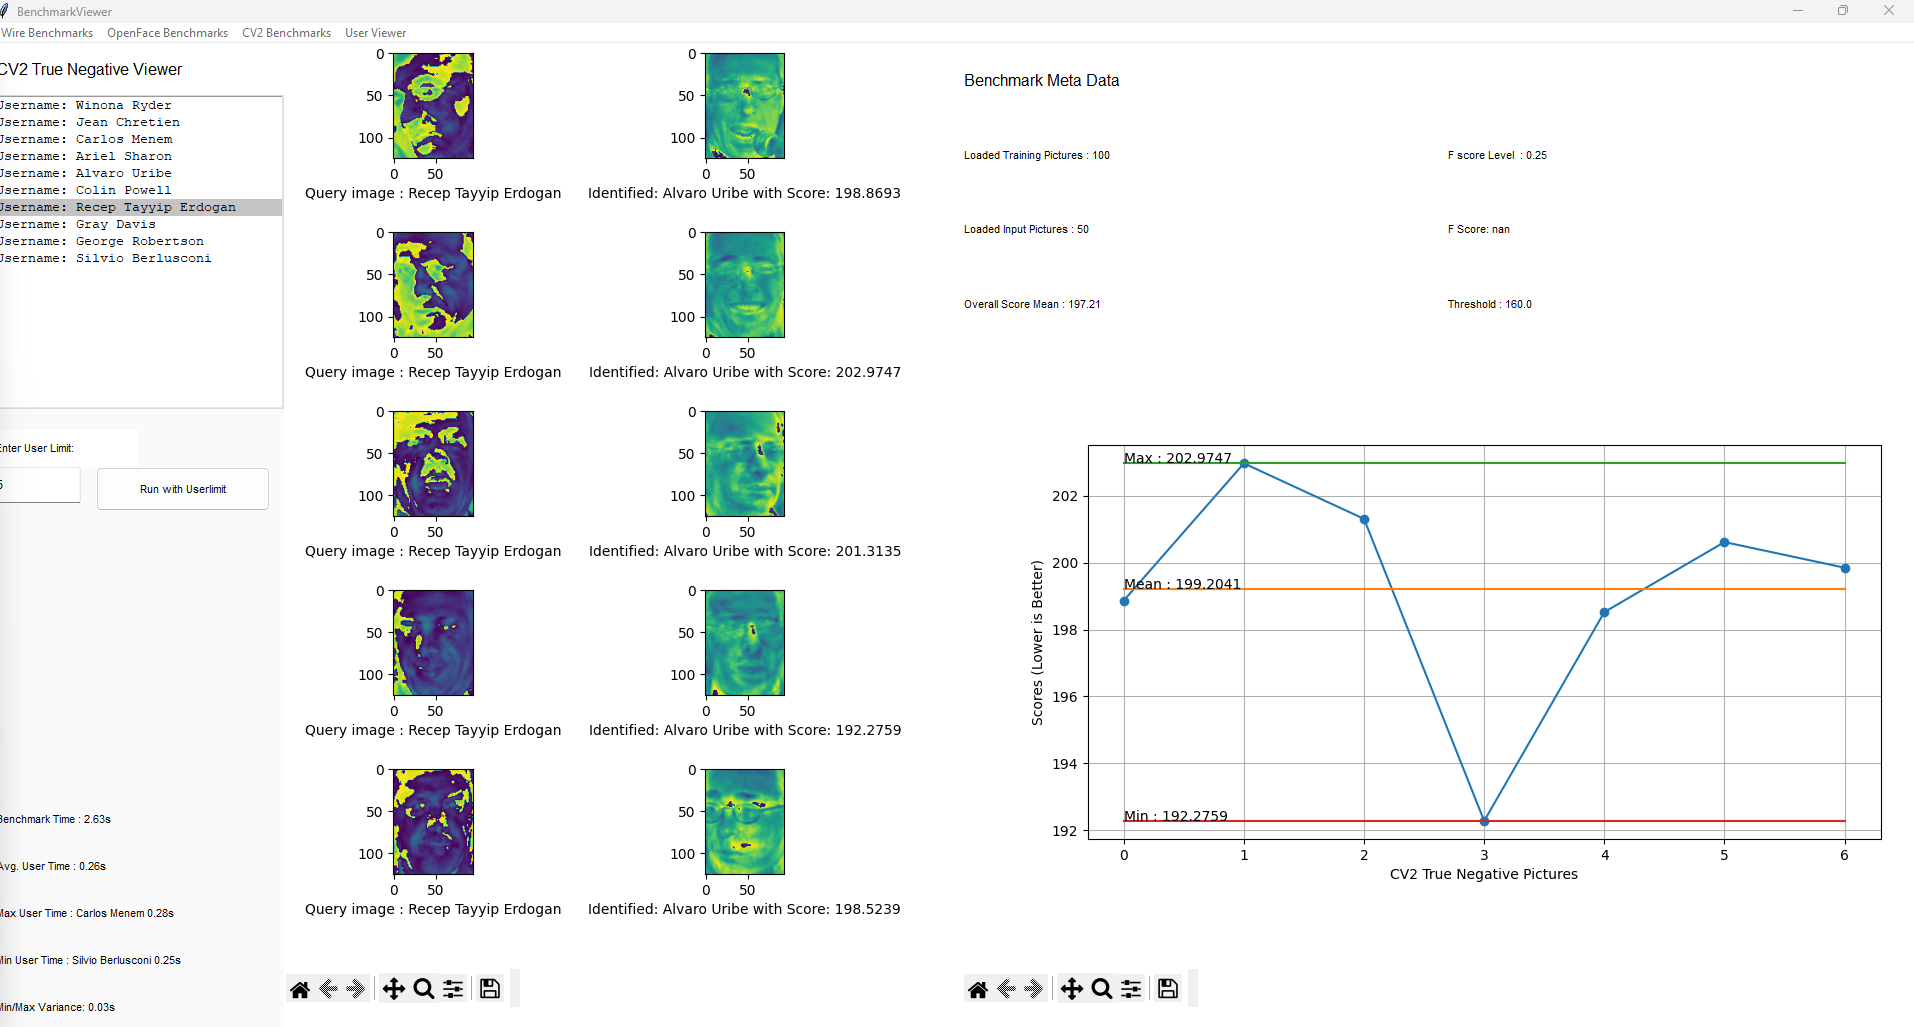
\includegraphics[scale=0.25]{images/benchmarking.png}
\end{center}
\end{frame}

\setbeamercolor{background canvas}{bg=blue!5}
\begin{frame}{}
\begin{center}
\Huge
Short demonstration
\end{center}
\end{frame}
\setbeamercolor{background canvas}{bg=white}

\begin{frame}{TODOs}
\begin{itemize}
    \item fix bug with f-scores
    \item extend benchmarking for implementation of logic group
    \item maybe: use more\slash{}different test and training data
\end{itemize}
\end{frame}

\setbeamercolor{background canvas}{bg=blue!20}
\begin{frame}{}
\begin{center}
\Huge
Any Questions?
\end{center}
\end{frame}

\end{document}

